\documentclass[a4paper,11pt]{article}
\usepackage{a4wide}
\usepackage{fullpage}
\usepackage[utf8x]{inputenc}
\usepackage[slovene]{babel}
\selectlanguage{slovene}
\usepackage[toc,page]{appendix}
\usepackage[pdftex]{graphicx} % za slike
\usepackage{setspace}
\usepackage{color}
\definecolor{light-gray}{gray}{0.95}
\usepackage{listings} % za vključevanje kode
\usepackage{hyperref}
\renewcommand{\baselinestretch}{1.2} % za boljšo berljivost večji razmak
\renewcommand{\appendixpagename}{Priloge}


\begin{document}
\label{naslov}
\pdfbookmark[1]{Naslov}{naslov}
\thispagestyle{empty}

\begin{center}
\begin{Large}
Modeliranje računalniških omrežij\\
Študijsko leto 2016/2017\\
\end{Large}

\vspace*{4cm}
\begin{LARGE}
\textbf{Strežniki s prioritetno čakalno vrsto\\}
\center{tema 5}
\end{LARGE}
\vspace*{0.5cm}

\begin{Large}
Končno poročilo 1. seminarske naloge\\

\vspace*{4cm}

David Rubin in Tilen Venko\\
Vpisni št. 63140229 in 63140280\\

\vspace*{5cm}
Ljubljana, \today
\end{Large}
\end{center}

\pagebreak
\setcounter{page}{1}
\pagenumbering{arabic}


\label{Kazalo}
\pdfbookmark[1]{Kazalo}{Kazalo}
\tableofcontents
\thispagestyle{empty}
\pagebreak

\section{Uvod in motivacija}

V simulacijskem orodju 	Omnet++ sva morala realizirati omrežje, ki je podano na sliki, pri čemer pa sva moral zajeti tri simulacije.
\begin{itemize}
  \item V prvem scenariju ima M/M/c prioritetno vrsto, paketi pa prioritete od 1 do 			10, čas strežbe v sekundah pa je enak prioriteti paketa. 
  \item V drugem scenariju je čas strežbe M/M/c poraydeljen normalno med 1s in 2s, 				čas strežbe M/M/1 pa je konstanten. Source proizvaja paketke z normalni 				porazdelitvijo. Switch1 pa dodeljuje paketke naključno.
  \item tretji scenarij je enak drugemo z izjemo tega, da Switch1 dodeljuje paketke 			po principu "least busy queue first".
\end{itemize}

\begin{figure}[htbp]
\begin{center}
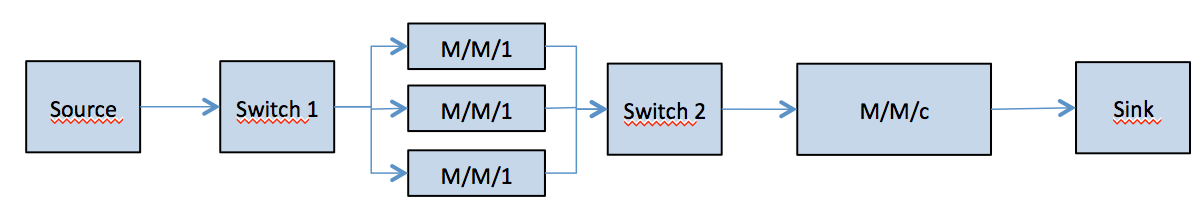
\includegraphics[scale=0.6]{shema.png}
\caption{shema omrežja, ki ga je potrebno realizirati.}
\label{Slika1}
\end{center}
\end{figure}

\section{Rešitev}

V simulacijskem okolju Omnet++ sva tako realizirala omrežje, ki je prikazano na spodnji sliki. Najina naloga je bila realizacija switchev in prilagoditev komponent Source, M/M/1 in M/M/c tako, da bodo delovali pravilno.
\begin{figure}[htbp]
\begin{center}
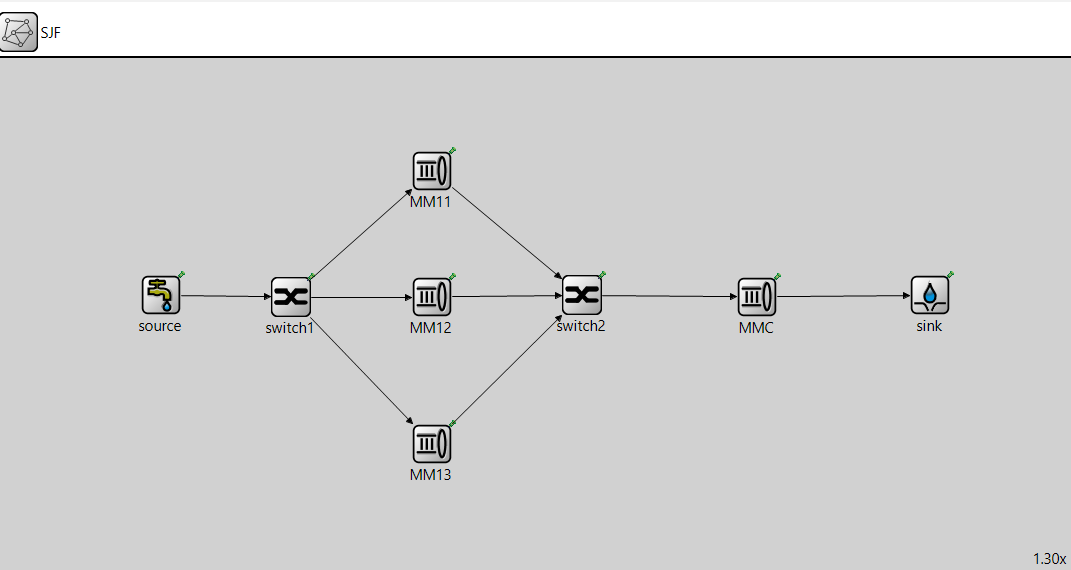
\includegraphics[scale=0.6]{omrezje.png}
\caption{shema omrežja realiziranega v ned datoteki.}
\label{Slika2}
\end{center}
\end{figure}

\subsection{Switch}

Switch naredimo tako, da ob inicializaciji inicializiramo vrata switcha in način v katerem deluje. \\
V Switch funkciji pa nato preverimo še ali je število vrat večje od 1, saj s tem določimo ali gre za Switch1 oz. Switch2. Če ugotovimo, da gre za Switch1 dalje preverjamo ali je način nastavljen na nič, kar pomeni, da bomo paketke naprej na M/M/1 pošiljali po naključnem načinu ali po principu najmanj zasedena vrsta najprej. \\
Če ugotovimo, da je switch v načinu "random", samo pošljemo paketen naprej na naključen M/M/1. Če pa je v načinu "LBQF", pa pridobimo čakalne vrste vseh treh M/M/1, na sledeč način:
\begin{lstlisting}
    mm1Queue *mm11 = (mm1Queue *)(gate(2621440)->getNextGate()->getOwner());
    mm1Queue *mm12 = (mm1Queue *)(gate(2621441)->getNextGate()->getOwner());
    mm1Queue *mm13 = (mm1Queue *)(gate(2621442)->getNextGate()->getOwner());
\end{lstlisting}  

Nato iz vsake vrste pridobimo kapaciteto in dolžino, iz teh podatkov določimo M/M/1 z najmanj zasedeno vrsto in nanj pošljemo paketek. \\
Če je število vrat switcha enako 1, pomeni da gre za Switch2 in samo posredujemo paketen naprej skozi edina vrata.

\subsection{Source}

Ob inicializaciji Sourcu določimo začetni čas, končni čas s čemer specificiramo kako dolgo se bo simulacija izvajala in pa število in maksimalno število paketkov, ki jih lahko zgenerira na enkrat. \\
V glavni funkciji pa neto še določimo naj generira paketke s prioriteto, ki je naključna od 1 do 10. Te paketka pa pošlje skozi izhod.

\subsection{mm1Queue}

Ob inicalicaciji M/M/1 določimo kapaciteto čakalne vrste, čas strežbe in število paketkov včakalni vrsti, ki je enako 0. Določimo tudi način v katerem M/M/1 delujejo in sicer če je primer enak 0, potem je čas strežbe enak prioriteti paketa, če ne pa je čas strežbe konstanten, v našem primeru enak 0.8s \\
V programu najprej preverimo, če v obdelavi ni nobenega paketka. Če to drži pošljemo naslednji paketek v obdelovanje. Če pa je procesna enota zasedena, preverimo ali je še prostor v čakalni vrsti. Če je prosto paketek dodamo v čakalno vrsto in povečamo števec vrsti, k išteje koliko paketkov je v čakalni vrsti. Če ja pa se zgodi, da je število paketkov, ki čakajo v vrsti enako kapaciteti paketek zavržemo.

\subsection{mmcQueue}

Ob inicializaciji določimo kapaciteto vrste, število paketov v vsrti, ki je enako 0, čas strežbe in način v katerem deluje. Če je način enak 0 potem paketke strežemo po njihovi prioriteti, v nasprotnem primeru pa tako, kot so prišli v vrsto.\\
Spet preverimo ali je prišlo novo sporočilo in če je katera od procesni enot prosta. V tem primeru vzamemo naslednji paket glede na način v katerem deluje M/M/c, torej ali po prioriteti ali pa naslednjega v vrsti. Če pa so vse procesne enote zasedene postaimo paket v vrsto, če je v njej še prostor. V nasprotnem primeru pa paketek zavržemo.

\section{Simulacije in rezultati}
Najprej sva simulirala primer, kjer gre za normalno delovanje in ne prihaja do nasičenj. Dolžina vrste MMCja je bila 100, hitrost porajanja paketkov pa je bila normalno porazdeljena med 1 in 2 sekundama. Število procesnih enot pa je enako 3. Pri tej simulaciji se v vrsti MMCja ni izgubil noben paketek porazdelitev čakanja v čakalni vrsti glede na prioriteto pa je vidna na spodnji sliki.\\
\begin{figure}[ht]
\begin{center}
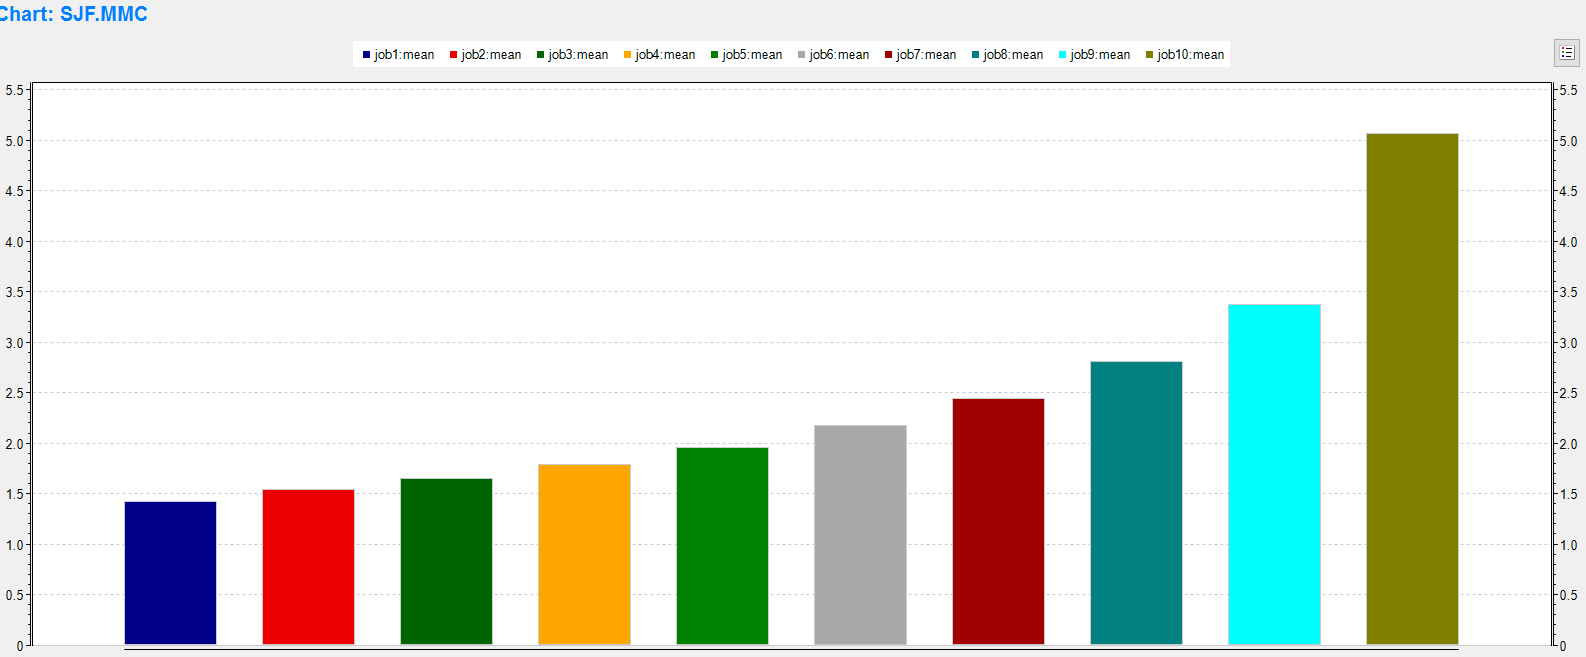
\includegraphics[scale=0.4]{queue100.png}
\caption{porazdelitev čakanja v vrsti glede na prioriteto paketa, merjeno v sekundah}
\label{Slika2}
\end{center}
\end{figure}
\\
Nato sva simulirala primer nasičenega omrežja. Kjer sva pustila vse parametre nespremenjene, samo čakalno vrsto sva zmanjšala na 3. Sedaj se je veliko paketkov izgubilo, se je pa pričakovano zmanjšal povprečni čakalni čas bivanja paketka v vrsti.\\
\begin{figure}[ht]
\begin{center}
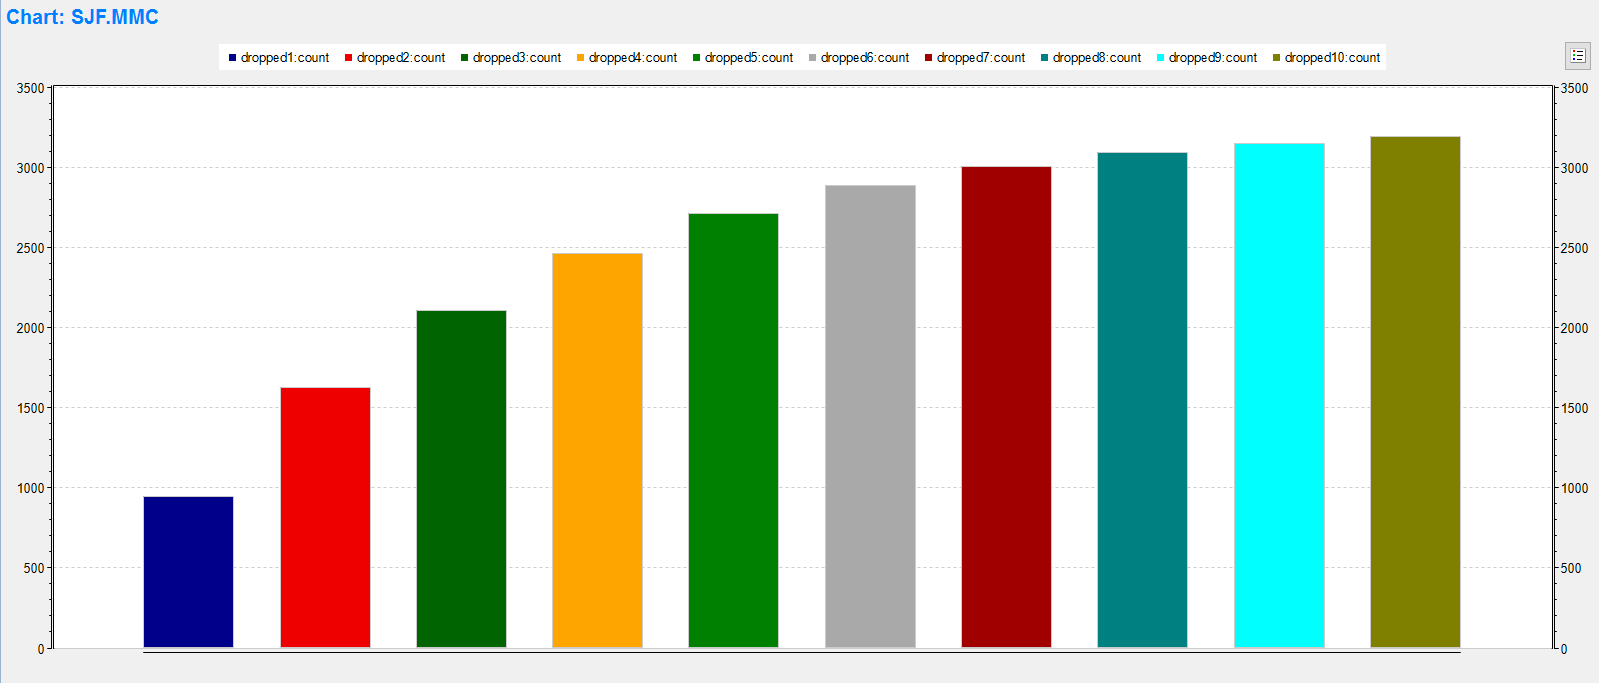
\includegraphics[scale=0.4]{dropped-queue3.png}
\caption{porazdelitev števila izgubljanih paketov glede na njegovo prioriteto}
\label{Slika2}
\end{center}
\end{figure}
\\
\begin{figure}[ht]
\begin{center}
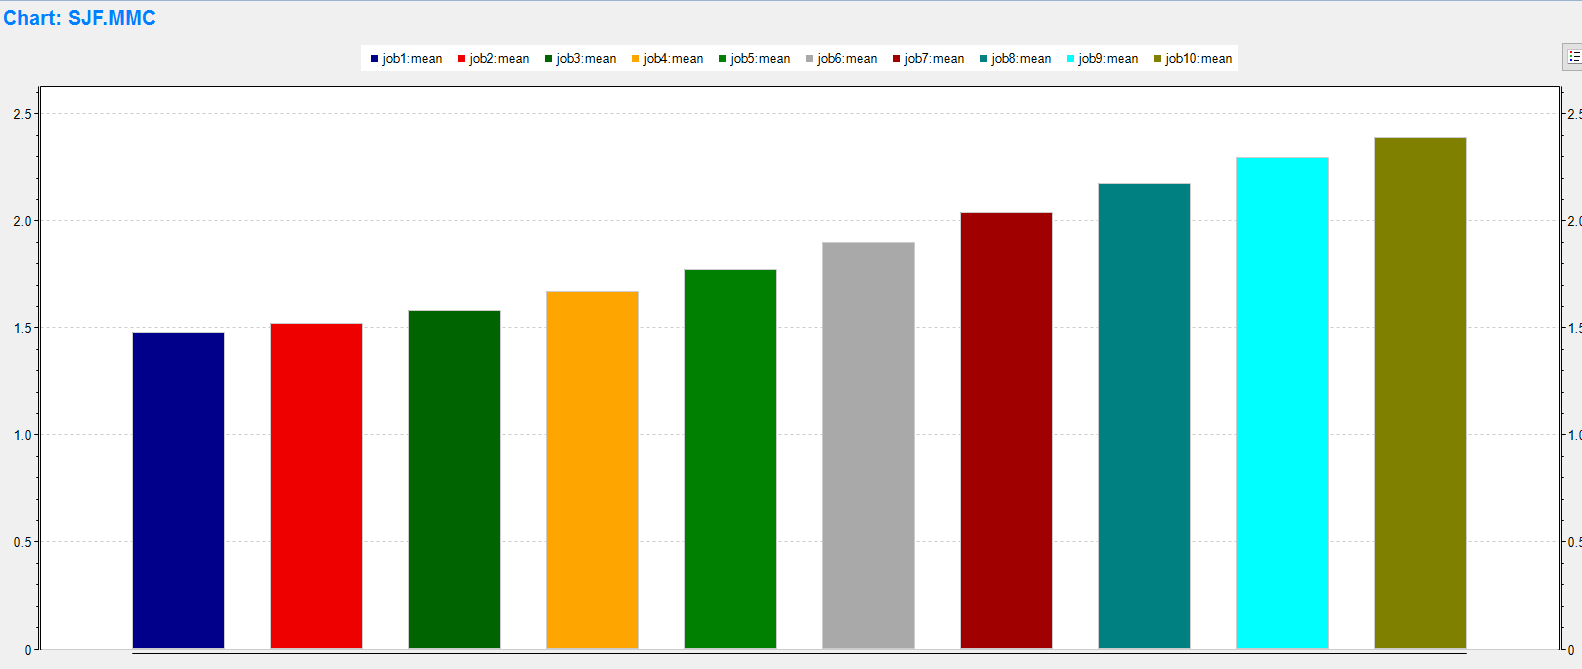
\includegraphics[scale=0.4]{queue3.png}
\caption{porazdelitev čakanja v vrsti glede na prioriteto paketa, merjeno v sekundah}
\label{Slika2}
\end{center}
\end{figure}
\\
\\
Sledil je še poskus, kaj se zgodi če zmanjšava čas porajanja paketov na normalno porazdelitev med 0.1s in 0.2s. Vendar so rezultati in grafi ostali nespremenjeni. Torej čas porajanja zahtevko ne vpliva na čakalni čas in izgubljanje paketov.\\
Za zadnjo simulacijo sva spremanila še število procesnih enot na 5, dolžina čakalne vrste je bila 3, čas porajanja paketkov pa normalno porazdeljen med 1s in 2s. Tu se paketki skoraj niso izgubljali, največ se jih je izgubilo paketkov s prioriteto 10 in to povprečno 7. Prav tako pa se je zelo znižal čas bivanja paketkov v čakalni vrsti.\\
\begin{figure}[ht]
\begin{center}
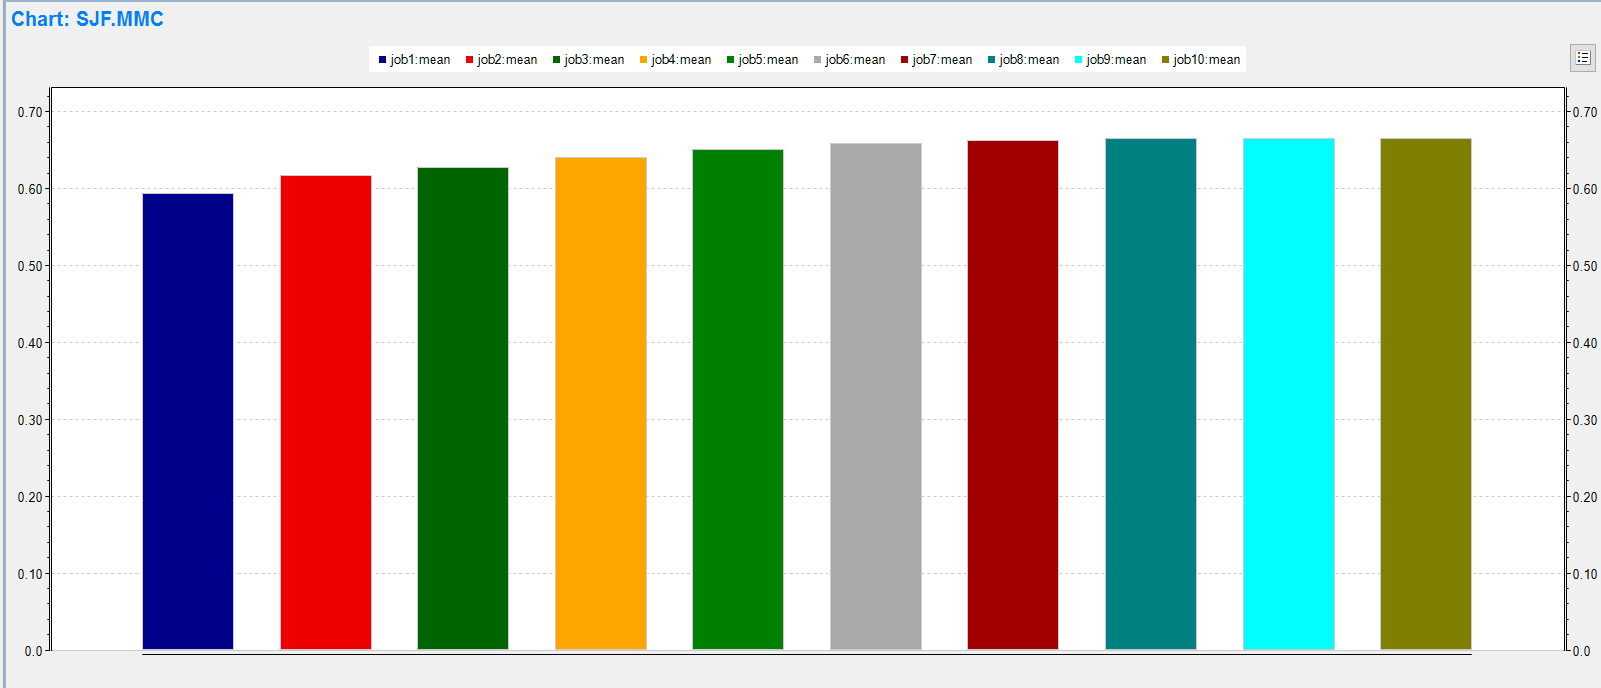
\includegraphics[scale=0.4]{queueu3-resource5.png}
\caption{porazdelitev čakanja v vrsti glede na prioriteto paketa, merjeno v sekundah}
\label{Slika2}
\end{center}
\end{figure}


\section{Zaključek}
Ugotovila sva, da na čas bivanja paketkov v čakalni vrsti in številu paketkov, ki se zavržejo najbolj vpliva število procesnih enot, pomembno pa na to vpliva tudi dolžina čakalne vrste. Med tem, ko hitrost porajanja zehtevkov nima vpliva na to, saj se že vsi paketki izgubijo v MM1. Čas čakanja v čakalni vrsti je pričakovano daljši, če ima paket višjo prioriteto. 

\pagebreak
\bibliographystyle{plain}
\bibliography{references}

\end{document}